\documentclass[tikz, border=1pt]{standalone}
\usepackage{cmap}
\usepackage[defaultsans]{droidsans}
\renewcommand*\familydefault{\sfdefault} %% Only if the base font of the document is to be typewriter style
\usepackage[T2A]{fontenc}
\usepackage[utf8x]{inputenc}
\usepackage{pgfplots}
\usepackage{pgfplotstable}
\usepackage{xcolor}
\usepackage{amsmath,amssymb}
\usepackage{esdiff,esint}
\pgfplotsset{compat=newest}
\usepgfplotslibrary{polar}
\usepgfplotslibrary{fillbetween}
\usetikzlibrary{decorations.markings, patterns}

\definecolor{ochre}{HTML}{e2431e} % #e2431e 0
\definecolor{lightorange}{HTML}{e7711b} % #e7711b 1
\definecolor{lightyellow}{HTML}{f1ca3a} % #f1ca3a 2
\definecolor{lightgreen}{HTML}{6f9654} % #6f9654 3
\definecolor{osci}{HTML}{82FF27}%#82FF27
\definecolor{sky}{HTML}{1c91c0} % #1c91c0 4
\definecolor{violet}{HTML}{43459d} % #43459d 5

\tikzset{
	lin/.style={
			line width=0.8pt,
			mark=none,
			black
		},
}

\pgfplotsset{
	every axis/.append style={
			line width=0.7pt,
			no markers,
			scale=0.7
		},
	error bars/.cd={
			y dir = both,
			y explicit
		}
}
\tikzset{
	line/.style={
			smooth, solid
		}
}

\tikzset{
  pics/carc/.style args={#1:#2:#3}{
    code={
      \draw[pic actions] (#1:#3) arc(#1:#2:#3);
    }
  }
}
\definecolor{c0}{HTML}{1f77b4}
\definecolor{c1}{HTML}{ff7f0e}
\definecolor{c2}{HTML}{2ca02c}
\definecolor{c3}{HTML}{d62728}

\definecolor{redd}{HTML}{fd0054}
\definecolor{blueb}{HTML}{509aaf}
\usepgfplotslibrary{fillbetween}

\begin{document}
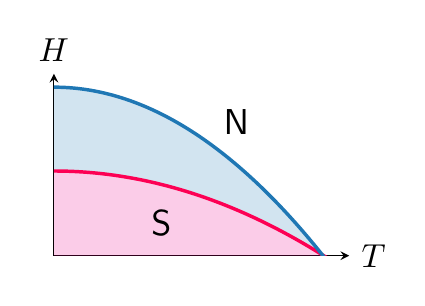
\begin{tikzpicture}
	\begin{axis}[
			% scale=0.7,
			axis lines=middle,
			xlabel={$T$},
			ylabel={$H$},
			major grid style={line width=.5pt,draw=black!70, dashed},
			% xtick distance=1,
			% ytick distance=1,
			xtick={0},ytick={0},
			xmin = 0,
			xmax = 0.55,
			ymin= 0.005,
			ymax= 1.09,
			width=12cm,
			height=8cm,
			% extra x ticks={-1.2},
			extra x tick style={
					grid=major,
					black, scale=1.2
				},
			extra x tick labels={
					{u=I}
				},
			scale=0.36,
			black!60,
			% grid=both,
			% x axis line style={ line width=0.5pt,},%yshift=1.2cm,
			% y axis line style={-},
			line width=0.75pt,
			xlabel style={black, scale=1.2,right},%yshift=1.2cm,
			ylabel style={black, scale=1.2,above},%yshift=1.2cm,
			% ylabel style={black, scale=1.2,xshift=-2.2cm,yshift=0.5em},%xshift=0.7cm,
		]
		% \begin{scope}
		% \coordinate (jn0) at (axis cs:0,0.24);
		% \coordinate (jn1) at (axis cs:1,0.24);

		% \draw[blueb, line width=1.25pt] (jn0) -- (jn1);	

		% \addplot+[
		% 	name path=B, samples=200, domain=0:0.8,
		% 	violet,
		% 	mark=none,
		% 	redd,
		% 	% densely dashed,
		% 	line width=1.25pt
		% 	% draw=none,
		% ] {0.4*(1-(x/0.8)^2)+0.01 };
		% % \addplot +[ redd,densely dashed,line width=1.25pt] plot table[x=x,y=z] {../data/12.out};
		% \addplot +[black,line width=1.25pt,dotted] plot table[x=x,y=y] {../data/3.out};

		% \addplot +[black,line width=1.25pt] plot table[x=x,y=y] {../data/12.out};
		% % \draw[
		% % 	violet,
		% % 	decoration={markings,mark=at position 1 with {\arrow[scale=1.5, rotate=-0,thick]{latex};},},   postaction={decorate}]
		% % (axis cs: {-0.549},{-0.631}) -- (axis cs: {2.097},{-0.631});
		% % \draw[
		% % 	violet,
		% % 	decoration={markings,mark=at position 1 with {\arrow[scale=1.5, rotate=-0,thick]{latex};},},   postaction={decorate}]
		% % (axis cs: {1.215},{2.1126}) -- (axis cs: {-1.4305},{2.1126});
		% % \draw[
		% % 	name path=A,draw=none
		% % ]
		% % (axis cs: {2.2},{-1.5})--(axis cs: {-1.2},{-1.5}) ;


		% \coordinate (Tc) at (axis cs:0.8,0.015);
		% \coordinate (rho) at (axis cs:1,1);
		% \coordinate (p3w) at (axis cs:0.525,1);
		% \coordinate (p0) at (axis cs:0.525,0.24+0.01);
		% \coordinate (jkr) at (axis cs:0,0.4);

		% \end{scope}
		% \addplot[name path=f,domain=-.15:1.05,blue] {x^2};

	    \path[name path=axis] (axis cs:0,0) -- (axis cs:1,0);

		\addplot+[
			name path=f, samples=200, domain=0:0.8,
			mark=none,redd,	line width=1.25pt
		] {0.5*(1-(x/0.5)^2)+0.01 };

		\addplot+[
			name path=f1, samples=200, domain=0:0.8,
			mark=none,c0,	line width=1.25pt
		] {1*(1-(x/0.5)^2)+0.01 };

		% \addplot+[
		% 	name path=f2, samples=200, domain=0:0.8,
		% 	mark=none,c1,	line width=1.25pt
		% ] {1*(1-(x/0.8)^2)+0.01 };

	    \addplot [fill=magenta,fill opacity=0.2] fill between[of=f and axis,soft clip={domain=0:1},];
	    \addplot [fill=c0,fill opacity=0.2] fill between[of=f1 and f,soft clip={domain=0:1},];
	    % \addplot [fill=magenta,fill opacity=0.2] fill between[of=f2 and axis,soft clip={domain=0:1},];

	    \draw (axis cs: {0.2},{0.2}) node[black,scale=1.3] {S};
	    \draw (axis cs: {0.34},{0.8}) node[black,scale=1.3] {N};

	\end{axis}
		% \draw[fill=black, black] (Tc) circle (2pt) node [below] {$T_c$};			
		% \draw[] (rho) node [above,c3!30!black] {$\rho(T)$};			
		% \draw[] (p3w) node [above] {$P_{3\omega}(T)$};			
		% \draw[] (jkr) node [left,c0!30!black] {$j_c(T)$};	

		% \draw[dashed,black!30] (p0) -- (p3w);	
		% \draw (jn0) node[left] {$j_\omega(T)$};	
\end{tikzpicture}
\end{document}